\documentclass[11pt]{article}
\usepackage[utf8]{inputenc,fullpage,authblk,indentfirst,graphicx,amsmath}
\setlength{\parindent}{5ex}
            
\title{Reciprocal Recommender Systems in Online Dating Systems}
\author[1]{Dailon Dolojan}
\affil[1]{Department of Computer Science, University of California Santa Cruz, Santa Cruz}

\date{March 17, 2018}

\begin{document}

\maketitle
\begin{center}
    \textbf{Abstract}
\end{center}

\indent A typical recommender system implements the concept of a user being recommended various items based off a user's interests. This system is commonly seen within online shopping which implements user-item recommendations to match items based off a user's interests. Although online dating sites utilizes the same process of recommending possible romantic partners similar to a typical recommender system, a successful match requires that the possible romantic partner reciprocate interest to the user. This concept of reciprocity of interest further distinguishes online dating sites as a reciprocal recommender system. Within this article, we will examine two reciprocal recommender systems and examine their approach to successfully matching online dating users with prospective relationship matches.
\pagebreak

\section{Introduction: What is a Reciprocal Recommender System?}

\indent Within the online dating industry, users create dating profiles in order to find potential romantic partners. Online dating sites often try to quantify ``human attractiveness" between a user profile and other site users through the usage of boolean expressions. These expressions are generated from user inputted data based on biographical information, and responses prompted from a dating site's questionnaire. The dating site utilizes the data from the user's profile to create suggestions of compatible partners through the site's matching algorithm.\\
\indent A recommender system is often defined as a system which provides a user with a generated set of items that the system perceives the user will like based on inputted data. Although the traditional definition of a recommender system works for recommending movies, books, or any inanimate item a user may want to buy online, the online dating industry contains another dimension of complexity such that the potential romantic partner who is paired with the user must also like the user in order to be considered a successful match. In traditional recommender systems such as online shopping, an individual can be suggested various shopping items without the pretense of these items needing to ``like" you back. This classifies online dating sites as a form of a reciprocal recommender system where not only the user has to like the recommended partner, but the recommended partner must also like the user to be classified as match.\\
\indent 
Within this article, we will examine various forms of recommender systems for online dating sites and compare the effectiveness of each system based off successful matches. 

\subsection{Recommender System's Online Dating Algorithms}

In analyzing reciprocal recommender systems, it is important to differentiate between two forms of algorithms that pair user and target profiles: content-based algorithms and collaborative filtering algorithms.

\subsubsection{Content-Based Filtering Algorithms}
 Content-based algorithms are algorithms that pair a user and potential partner by analyzing the data collected from user profiles and checking for similarities. The algorithm is based off the idea that if two users have similar content in their profiles, both users would be a successful match. 
 

\subsubsection{Collaborative Filtering Algorithms}
Conventional collaborative filtering algorithms used in recommender systems often recommend objects to users based on the idea that users with similar behavior will like the same objects. This form of filtering algorithm is often seen within e-commerce, but within the context of a reciprocal system collaborative filtering is implemented to recommend a user all other profiles whose recommendations also contain A.

\pagebreak

\section{RECON Recommender System 2010\footnote{Equations found in this section were obtained from \cite{RECON}}}
 Within ``RECON: A Reciprocal Recommender for Online Dating" (Luiz Pizzato et al. 2010), the authors of the article create a reciprocal recommender system that analyzes the interaction of a user's \textit{explicit}  and \textit{intrinsic} profiles of preferences within their ideal partner through content-based filtering algorithms \cite{RECON}. An \textit{explicit} profile is created by the user  where the individual provides information about themselves and their preferences explicitly. In comparison, an \textit{intrinsic} user profile is a profile of the user developed by the online dating site that collects information based on the user's behavior interacting with the recommender site. \\
 \indent In using a traditional online dating site, a user creates a profile filled with inputted biographical information about the individual as well as their perceived ideal partner. The site prompts the user to provide information such as age, gender, location, the type of relationship sought after, and other various attributes.The system will then recommend potential matches to the user where the user can then browse any of the profiles to determine if the person appears to be a viable match. The user can then send a pre-defined message asking if the individual is interested and exchange contact information.\\ 
 \indent As the user interacts with a multitude of profiles, the system will develop an \textit{intrinsic} history of his behavior on the site by examining the profiles the user decides to message. The system then uses the data collected from this \textit{intrinsic} profile to develop a preference model for the user. This preference model is composed of all the attributes found in a potential partner that a user decides to message and the attributes associated with the potential partners that received a positive reply from the user when the user is messaged first. The preferences generated by the site is then used to calculate compatibility with a potential partner. The compatibility scores of a potential partner is then compared amongst other potential matches to output a list of recommendation for the user.
 
 \subsection{User preference's}
 The online dating system creates user profiles with two key components that consist of free text information and a pre-defined list $A$ of attributes \cite{RECON}. The pre-defined list of attributes represent numeric and nominal attributes which are discretised into various attribute groups. An example of this can be seen with a user's age being discretised into age groups such as 22-24, 24-26, and so forth. \\
\indent A user $x$ will have a profile $U_x$ that will contain values $v$ of a specific attribute $a$ which is represented as
\begin{equation}
U_x= \{v_a: for\ all\ attributes\ a \in A\}
\end{equation}

The system then generates a list $M_x$ composed of potential partners that user $x$ has sent a message to:
\begin{equation}
M_x= \{m: m\ is\ a\ potential\ partner\ messaged\ by\ x\}
\end{equation}

Preference $p$ of a user $x$ with values of an attritbute $a$ where $n$ is the number of times $v$ has appeared in $M_x$ can then be represented by the following expression:
\begin{equation}
p_x_,_a = \{(v,n): for\ all\ unique\ discrete\ values\ v\ of\ a\}
\end{equation}

User $x$'s complete set $P_x$ of preferences can be expressed as a list of $p_x_,_a$ for every attribute $A$ such that
\begin{equation}
P_x = \{p_x_,_a:\ for\ all\ a\ \in A \}
\end{equation}

 \subsection{RECON's Algorithm}
 Once the preferences $P_x$ of a user $x$ is determined, RECON implements two algorithms to generate a list of recommendations. The system uses a compatibility algorithm to determine a numerical score of how well the user and the potential partner are suited for each other. After generating a list of compatibility scores with various partners, the system will implement a reciprocal recommendation algorithm. This algorithm creates a reciprocal score that reflects how well the user and the potential partner match according to their preferences and attributes.
 
 \subsubsection{Compatibility Algorithm}
 The compatibility score of a user and a potential partner is calculated using the following algorithm.
 
\begin{figure}[h]
\begin{center}
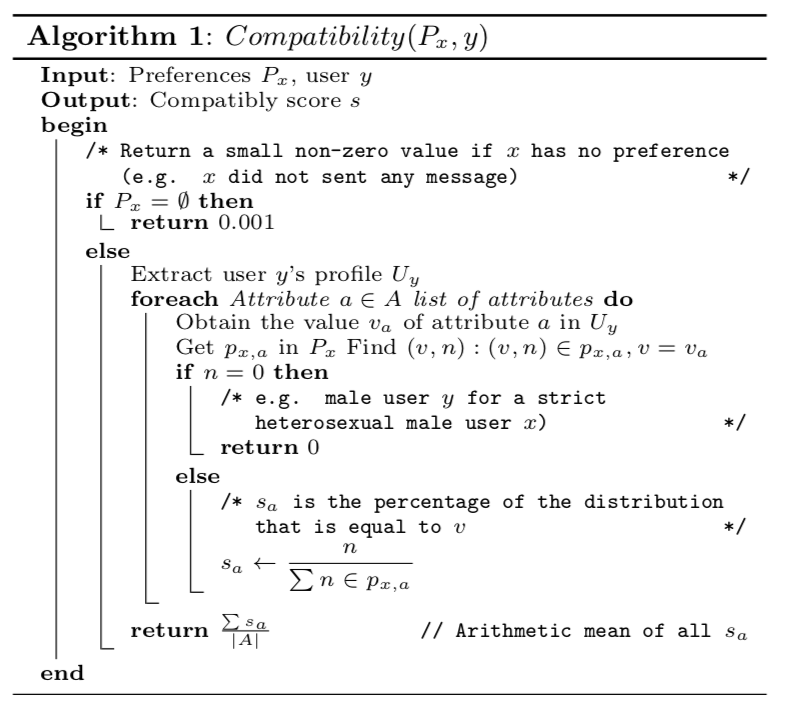
\includegraphics[width=10cm,height=10cm,keepaspectratio]{Recon_Alg1.png} 
\caption{RECON's algorithm to calculate Compatibility given a user $x$'s preferences $P_x$ and a user $y$ \cite{RECON}.}    
\end{center}
\end{figure}

\indent This algorithm takes user $x$'s preferences $P_x$ and a potential partner user $y$ as inputs to determine a compatability score $s$. The algorithm checks to see if user $x$ has no preferences such that $P_x = \emptyset$. If $P_x = \emptyset$, the compatibility score will result in 0.001. Otherwise, the algorithm will extract user $y$'s profile $U_y$ and obtain the values $v$ of every attribute $a$ within the list $A$ of attributes. If the number of times $n$ the value $v$ occurred within user $x$'s messaging list $M_x$ is equal to zero, then the output will be equal to zero. This illustrates that if an attribute $a$ does not appear within user $x$'s preferences $P_x$, the attribute will return an output of zero. If $n>0$ for an attribute $a$, the algorithm will calculate a compatibility score $s_a$ for that specific attribute by dividing $n$ from the overall sum of values that have appeared in $M_x$. For all $a \in A$, the algorithm finally calculates the arithmetic mean of all compatibility scores $s_a$ to determine overall compatibility such that the sum of $s_a$ is divided by the number $A$ of attributes.

 \subsubsection{Reciprocal Recommendation Algorithm}
  Once the compatibility score is obtained for a user $y$, RECON implements a reciprocal recommendation algorithm to calculate a score that illustrates how well the preferences of a user match with a potential partner's attributes and vice versa. The algorithm intakes a number $N$ of recommendations for user $x$ and outputs a list of recommendations $R$ with a list $S$ of reciprocal scores.

\begin{figure}[h]
\begin{center}
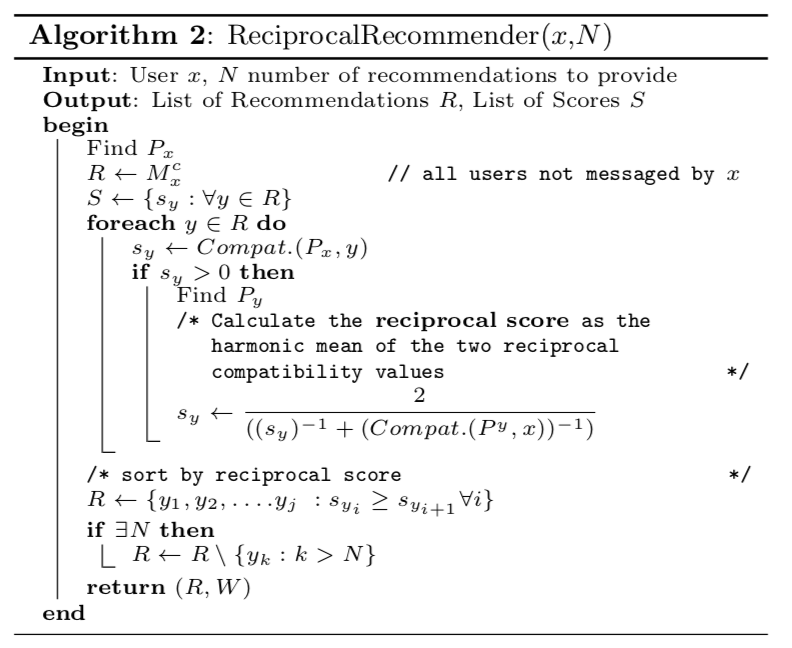
\includegraphics[width=10cm,height=10cm,keepaspectratio]{Recon_Alg2.png} 
\caption{RECON's algorithm to generate a list of recommendations \cite{RECON}.}    
\end{center}
\end{figure}

\indent The algorithm first determines user $x$'s preferences $P_x$, the set $R$ of recommendations that are comprised of the set $M_x^c$ of potential partners that have not been messaged by user $x$, and the set $S$ of reciprocal scores. For every potential partner $y\ \in R$, the algorithm calculates the compatibility score then calculates the reciprocal score as ``the harmonic mean of the two reciprocal compatibility values" \cite{RECON}. The algorithm then sorts the potential partners based on the highest reciprocal scores and returns the sorted list $R$.

 \subsection{Analysis of RECON}
\indent Although RECON's recommendation algorithm has a linear performance, implementing RECON within a database of all users would result in a $O$($N^2$)  time complexity \cite{RECON}. Therefore to accurately test the RECON system, the team chose to use a smaller set of users. The set was comprised of users who are ``of the dominant gender, who are within one standard deviation of mean age, and who live one standard deviation from the mean location" (Pizzato et al). \\
\indent The two main goals set out by RECON were to understand ``the role of reciprocity in the effectiveness of the algorithm" (Pizzato et al) and ``how well RECON performs when it is restricted in the number of recommendations it can offer" (Ibid.). \\
\indent In order to test the efficiency of the RECON recommender system, the users' message history was collected throughout a six week time period. The first four weeks were used as training data to allow for the content based recommender system to build an \textit{intrinsic} profile of the user and determine matches whereas the last two weeks were used to test the RECON system. Within the training set of data, 90,000 users sent approximately 1.4 million messages.\\
\indent RECON's success was then measured by the \textit{success rate} of \textit{known} interactions $pr$ that have occurred with the list of sorted recommendations throughout the test period. The success rate of user $x$'s list of recommendations $R$ is the ''proportion of the \textit{known} interactions [$kr$] (users messaged by $x$) that were positive (users who replied to $x$ positively".
\begin{equation}
Success(x,R) = \frac{\lvert\{pr:\ pr\ \in R,\ pr\ replied\ positively\ to\ x\} \rvert}{\lvert \{kr:\ kr\ \in\ R,\ kr\ \in\ M_z\ \} \rvert}\\
\end{equation}

\indent The experiment also measured \textit{recall} which is ``the proportion of known interactions that were present in the list of recommendations over all positive interactions [$py$] made by a particular user" (Pizatto et al.).
\begin{equation}
Recall(x,R) = \frac{\lvert\{pr:\ pr\ \in R,\ pr\ replied\ positively\ to\ x\} \rvert}{\lvert \{py:\ py\ \in\ M_x,\ replied\ positively\ to\ x\} \rvert}
\end{equation}

For example, if user $x$ had a list of the top 5 recommendations where user $x$ messaged only two potential partners within the recommended list, then RECON's algorithm will only calculate the success rate and recall based on these two interactions. Consider a scenario where user $x$ obtains ten positive replies within the testing period such that $py=10$ where only two known interactions occur meaning $kr=2$. If only one of those interactions is positive $pr=1$, the success rate would be 50\% and recall would be 10\%.

\subsection{Results}

\begin{figure}[h]
\begin{center}
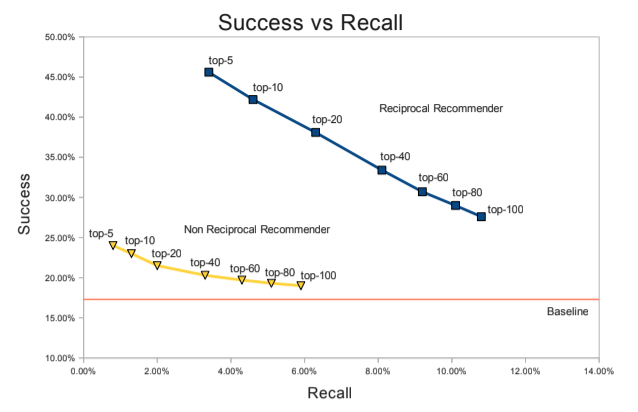
\includegraphics[width=10cm,height=10cm,keepaspectratio]{Recon_Results.png} 
\caption{Comparing the success rate and recall between reciprocal recommender, non-reciprocal recommender, and the use of neither \cite{RECON}.}    
\end{center}
\end{figure}

The article presents its findings by comparing the success rate and recall for RECON against a non-reciprocal recommender system with varying sizes of the number of recommendations. A baseline success measure of 17.3\% was determined by the proportion of messages sent by users that received a positive reply within the testing set \cite{RECON} without receiving recommendations from any recommendation system.\\
\indent Given a list of top 10 recommendations, the reciprocal recommender has a 42\% success rate and 4\% recall whereas the non-reciprocal recommender has a 23\% success rate and 1\% recall. This trend in improvement of success rate and recall can be seen for varying sizes of recommendation lists thus providing evidence that reciprocity is essential to recommender systems which require two individuals to have a mutual interest.

\section{Peng Xia et al's Reciprocal Recommendation System for Online Dating\footnote{Equations found in this section were obtained from \cite{recip}}}
In ``Reciprocal Recommendation System for Online Dating" (Peng Xia et al), the authors develop a recommendation system based off of RECON that utilizes both content-based and collaborative filtering-based algorithms to measure compatibility between users. The goal of the recommendation system is to recommend users who have a mutual interest as well as a higher likelihood of messaging each other. The design of this recommendation system is based in four components: extraction of user based features, extraction of graph based features, computation of similarity and reciprocal scores, and generation of a recommended user list \cite{recip}.

\subsection{The Design of Recommender System}
\subsubsection{Extraction of User Based Features}
The user must first create a profile that is comprised of various information such as gender, age, height, weight and other categorical attributes. The recommender system implements the same user preference model and compatibility algorithm described in RECON  \cite{RECON}.\\
\indent In addition, the recommender system includes a second compatibility equation to include ``numerical attribute information that are compared between the boundaries of continuous ranges" \cite{recip}. This second compatibility equation is included due to RECON's inability to compare two users that do not fall within the same categorical group. An example of this can be seen when comparing a 19 year old user that falls within the 18-20 range and a 21 year old user that falls within the 20-22. The recommender system modifies RECON's original equation by representing the maximum absolute difference for an attribute $a$ with a value $v$ among all users when comparing user $i$ and $j$.

\begin{equation}
    v_a^* = max_{i \neq j} \lvert v_a^i-v_a^j\rvert
\end{equation}

Equation 7 is then used to calculate the value of a specific attribute given $v_a^*$ where $Q_a(x,y)$ represents the value of numeric attributes.

\begin{equation}
    Q_a(x,y)= \frac{v_a^* - \lvert v_a^x-v_a^y\rvert}{v_a^*}
\end{equation}

The overall content similarity of user $x$ and user $y$ with their respective attribute sets $A_x$ and $A_y$ is then calculated by following equation:

\begin{equation}
content\ similarity(x,y) = \frac{\sum_{a \in A_x \cap A_y}Q_a(x,y)}{\lvert A_x \cap A_y \rvert}
\end{equation}

\subsubsection{Extraction of Graph Based Features}
The online dating site used within this study can be represented as a bipartite network between men and women. Graph-based similarity features are then derived from the bipartite graph to indicate a user's active level in dating and attractiveness \cite{recip}. 

\indent The recommender system calculates interest similarity and attractiveness similarity through message history between users. The article defines the set $Se(x)$ as the set of messages user $x$ has sent to user $y$. 
\begin{equation}
    Se(x) = \{y: x\ has\ sent\ a\ message\ to\ y\}
\end{equation}

The set $Re(x)$ is defined as the set of messages user $x$ has received from user $y$.

\begin{equation}
    Re(x) = \{y: x\ has\ received\ a\ message\ to\ y\}
\end{equation}

From these two sets, we can define the interest similarity between two same-sex users $x$ and $y$ as the fraction of users both $x$ and $y$ messaged over the set of all users that $x$ and $y$ messaged.

\begin{equation}
    interest\ similarity(x,y) = \frac{\lvert Se(x) \cap Se(y) \rvert}{\lvert Se(x) \cup Se(y) \rvert}
\end{equation}

Attractiveness similarity can be defined as the fraction of the set of users that both users $x$ and $y$ received messages from over the set of all users that messaged either user $x$ or $y$.

\begin{equation}
    attractiveness\ similarity(x,y) = \frac{\lvert Re(x) \cap Re(y) \rvert}{\lvert Re(x) \cup Re(y) \rvert}
\end{equation}


\subsubsection{Computation of Similarity and  Reciprocal Scores}
A reciprocal score of two users is calculated using the similarity equations derived from the user-based and graph-based features. The algorithm illustrated in \textbf{Figure 4} demonstrates how a reciprocal score is calculated.
Within this algorithm, compatibility scores are calculated based on the similarity of neighbor sets that the user is associated with. $Neighbor_1$() illustrates the  set of users that $x$ has sent messages to whereas $Neighbor_2$ illustrates the set of users that $y$ has sent messages to. In addition, $Similarity_1$(,) and $Similarity_2$(,) are functions that determine overall similarity between a pair of users. The algorithm calculates $s(x, y)$ as the measure of similarity between user $x$ and user $y$ where the reciprocal score is the harmonic mean of both $s(x,y)$ and $s(y,x)$.

\subsubsection{Generate Recommended User List} For every user within the online dating site, a recommendation list is created that ranks reciprocal scores for top-$N$ users within a list.

\begin{figure}[h]
\begin{center}
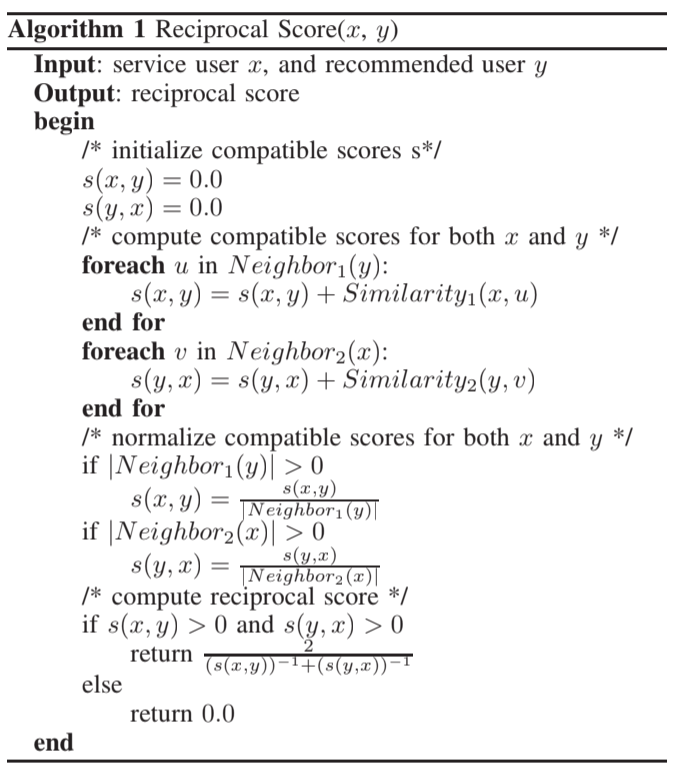
\includegraphics[width=10cm,height=10cm,keepaspectratio]{Recip_Alg1.png} 
\caption{An algorithm that inputs a user $x$ and recommended user $y$ and returns the reciprocal score of a pairing. \cite{recip}.} 
\end{center}
\end{figure}

\section{Analysis}
Within the article, the recommender system is evaluated by ''comparing the top-N users
in the recommended list with the receivers contacted by the service user in test set." \cite{recip}. There are three sets of potential partners defined per user.
Set $T$ is the set of potential partners recommended to the user, set $I$ is the set of potential partners messaged by the user, and set $R$ is the set of potential partners that have been messaged by the user. From these sets, the authors define I-Precision and I-Recall to ``measure an algorithm’s performance in recommending users that the service user is interested in and thus likely to contact" \cite{recip}.  

\begin{equation}
    I-Precision = \frac{\lvert I \cap T\rvert}{T}, I-Recall = \frac{\lvert I \cap T\rvert}{I}
\end{equation}

Whereas R-Precision and R-Recall ``measure an algorithm’s performance in recommending users who have mutual interest with the service user and are thus likely to reciprocate when contacted" \cite{recip}.

\begin{equation}
    R-Precision = \frac{\lvert R \cap T\rvert}{T}, R-Recall = \frac{\lvert R \cap T\rvert}{R}
\end{equation}

\section{Conclusion}
Both articles exemplify viable recommender systems that provide functional top-N list of recommendations for a specific user. Although RECON illustrates a fundamental basis of reciprocity, the RECON system is limited in its implementation due to its inability to compare attributes of different discretised groups. Through the preservation of values of numeric attributes within the recommender system outlined by Peng Xia et al, the content based algorithm posed by Peng Xia et al outperforms RECON's algorithm in precision and recall. For simplification purposes, we will define RECON's content based algorithm as CB1 and Peng Xia et al's content based algorithm as CB2.

Figure 5 and Figure 6 display the performance in comparing CB1 and CB2 in recommending potential partners that the user is interested in. 

\begin{figure}[h]
\begin{center}
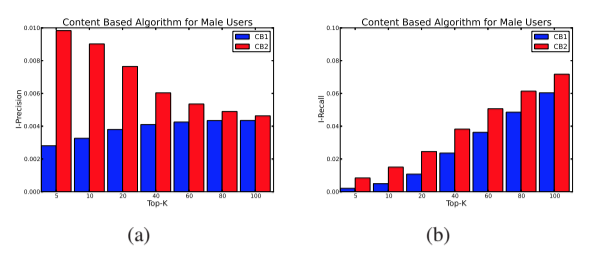
\includegraphics{i_male.png} 
\caption{Comparison of I-Precision and I-Recall between CB1 and CB2 for males \cite{recip}.} 
\end{center}
\end{figure}

\begin{figure}[h]
\begin{center}
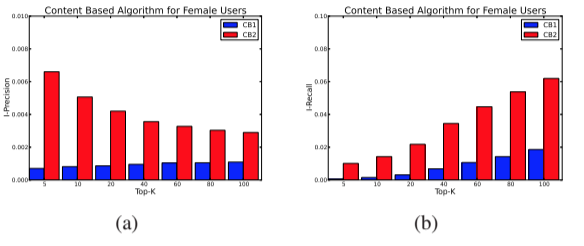
\includegraphics{i_female.png} 
\caption{Comparison of I-Precision and I-Recall between CB1 and CB2 for females. \cite{recip}.} 
\end{center}
\end{figure}

Figures 6 and 7 illustrate the performance of comparing CB1 and CB2 in recommending potential partners who will be messaged by the user.


\begin{figure}[h]
\begin{center}
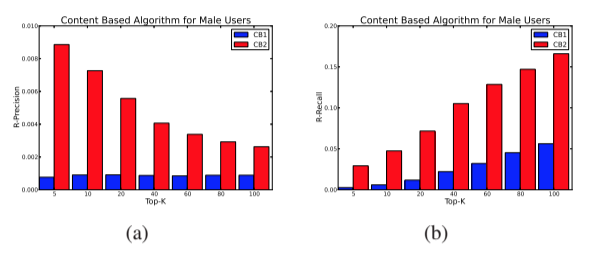
\includegraphics{r_male.png} 
\caption{Comparison of R-Precision and R-Recall between CB1 and CB2 for males\cite{recip}.} 
\end{center}
\end{figure}

\begin{figure}[h]
\begin{center}
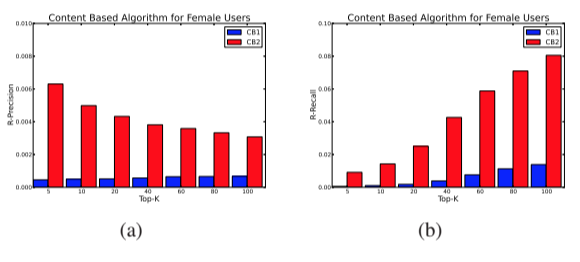
\includegraphics{r_female.png} 
\caption{Comparison of R-Precision and R-Recall between CB1 and CB2 for females \cite{recip}.} 
\end{center}
\end{figure}

\pagebreak
\nocite{*}
\bibliographystyle{plain}
\bibliography{mybib.bib}


\end{document}
